\documentclass[10pt,letterpaper]{article}
\usepackage{amsmath}
\usepackage{amsfonts}
\usepackage{amssymb}
\usepackage[english]{babel}
\usepackage{breakurl}
\usepackage[superscript]{cite}
% \usepackage{draftwatermark}
\usepackage{fancyhdr}
\usepackage{float}
\usepackage[margin=1in]{geometry}
\usepackage{graphicx}
\usepackage{hyperref}
\usepackage[utf8]{inputenc}
\usepackage{makeidx}
\usepackage{multicol}
\usepackage{nth}
\usepackage[default,scale=1.0]{opensans}
\usepackage{setspace}
\usepackage{siunitx}
\usepackage{svg}
\usepackage{subcaption}
\usepackage{tikz}
\usepackage{url}
\usepackage{kantlipsum}

%% Preamble
% Custom commands
\newcommand{\ts}{\textsubscript}

% Use hyphans to break up urls
\def\UrlBreaks{\do\/\do-}

% Draft watermark
% \SetWatermarkText{\textsc{Draft}}
% \SetWatermarkScale{5}

% PDF and href setup
% Hyper ref
\hypersetup{
	colorlinks=true,
	citecolor=black,
	linkcolor=black,
	filecolor=black,
	urlcolor=blue,
	pdftitle={Engineering Economic Analysis Report of Renewable Technologies},
	bookmarks=true
}
\urlstyle{same}

% Page semantics
\pagestyle{fancy}
\fancyhead[L]{\slshape\MakeUppercase{MECH 431}}
\fancyhead[R]{\slshape Muchen He}
\fancyfoot{}
\fancyfoot[C]{\thepage}

\parindent 0ex

% Meta
\author{Muchen He}
\title{Renewable Energy For Average Household in Edmonton}
\begin{document}
\begin{titlepage}
	\begin{center}
		\vspace*{3in}
		\line(1, 0){400}\\
		\Huge{\textbf{Renewable Energy For An Average Household in Edmonton}}\\[0.2cm]
		\large{\textbf{Engineering Economic Analysis Report of Renewable Technologies}}\\[1cm]
		\Large{\textbf{MECH 431}}\\
		\textbf{University of British Columbia}\\
		\line(1, 0){400}\\
		\vfill
		\Large{Muchen He}\\
		44638154\\

		\today\\
	\end{center}
\end{titlepage}

% Executive Summary
\section*{Summary}
\clearpage

% Table of contents
\setcounter{secnumdepth}{3}
\tableofcontents
\thispagestyle{empty}
\clearpage

% Uncomment for list of tables and figures
\thispagestyle{empty}
\listoffigures
\listoftables
\newpage

% Set page and section counter
\setcounter{page}{1}

\section{Introduction}\label{section:introduction}

\subsection{Problem}

Edmonton, being the "Oil city", the captial of the province whose major export is oil, is relying too much on non-renewanle resources like fossil fuel. Thus we need to take steps to move towards greener solutions.\\

Edmonton average household consumes an average of between 7500 to 8500 kWh per year. It would be world changing if all these electrical energy can be derived from renewable sources. With the rising prices of means to produce energy, the renewable approach could be economically viable.\\
\\
Alberta consumes more than 10,000 GWh of energy a year. This averages to about 2400 kWh per capita\cite{average-albertan-consumption}. The province has an over-reliance on non-renewable resources for its power generation. Furthermore, projects involving building pipelines and method of hydraulic fracturing (fracking) poses serious environmental impact\cite{fracking-kurzgesagt}.\\
\\
This report intends to explore the economic viablility of renewable solutions that an individual or a family can realistically implement.\\
\\

\subsection{Solution Overview}

To solve this problem, we will look at the economic analysis of solar solutions. The analysis outlines the economic criteria and economic viability of implementing solar generation for a single average household in the sub-urban neighbourhoods of Edmonton.\\
\\
An adequate sustainable solar system should take pressure off of drawing energy from the grid, the electric companies, whose energy is generated from natural gas, coal, and oil. The main parts to a solar system consists of three components\cite{components}:

\begin{enumerate}
	\item Generation: this includes the solar (or commonly referred to as PV) cells that converts photon energy from the sun into electrical voltages. In the context of analsis and design, this would also include the infrastructure setup for these cells, such as mechanical mounting racks, and installation efforts.
	\item Storage: this includes the necessary electrical equipment to ensure extra energy generated from the PV panels could be stored to be used or sold. 
	\item Utilization: this includes the delivery of energy, which consists of equipment to convert generated direct currents (DC) to household appliance compatible alternating current (AC), like an inverter. This component also considers metering the power output such that excess energy can be sold.
\end{enumerate}

\section{Design}

A template will be built from an average house loacted in Edmonton suburban area, I will use my house as a referece. The type of landscape and architecture is ubiquitous throughout Edmonton neighbourhood and thus would make the model adequate.\\
\\
The power analysis and simulation will be based off of this template.\\
\\

\begin{figure}[H]
	\centering
	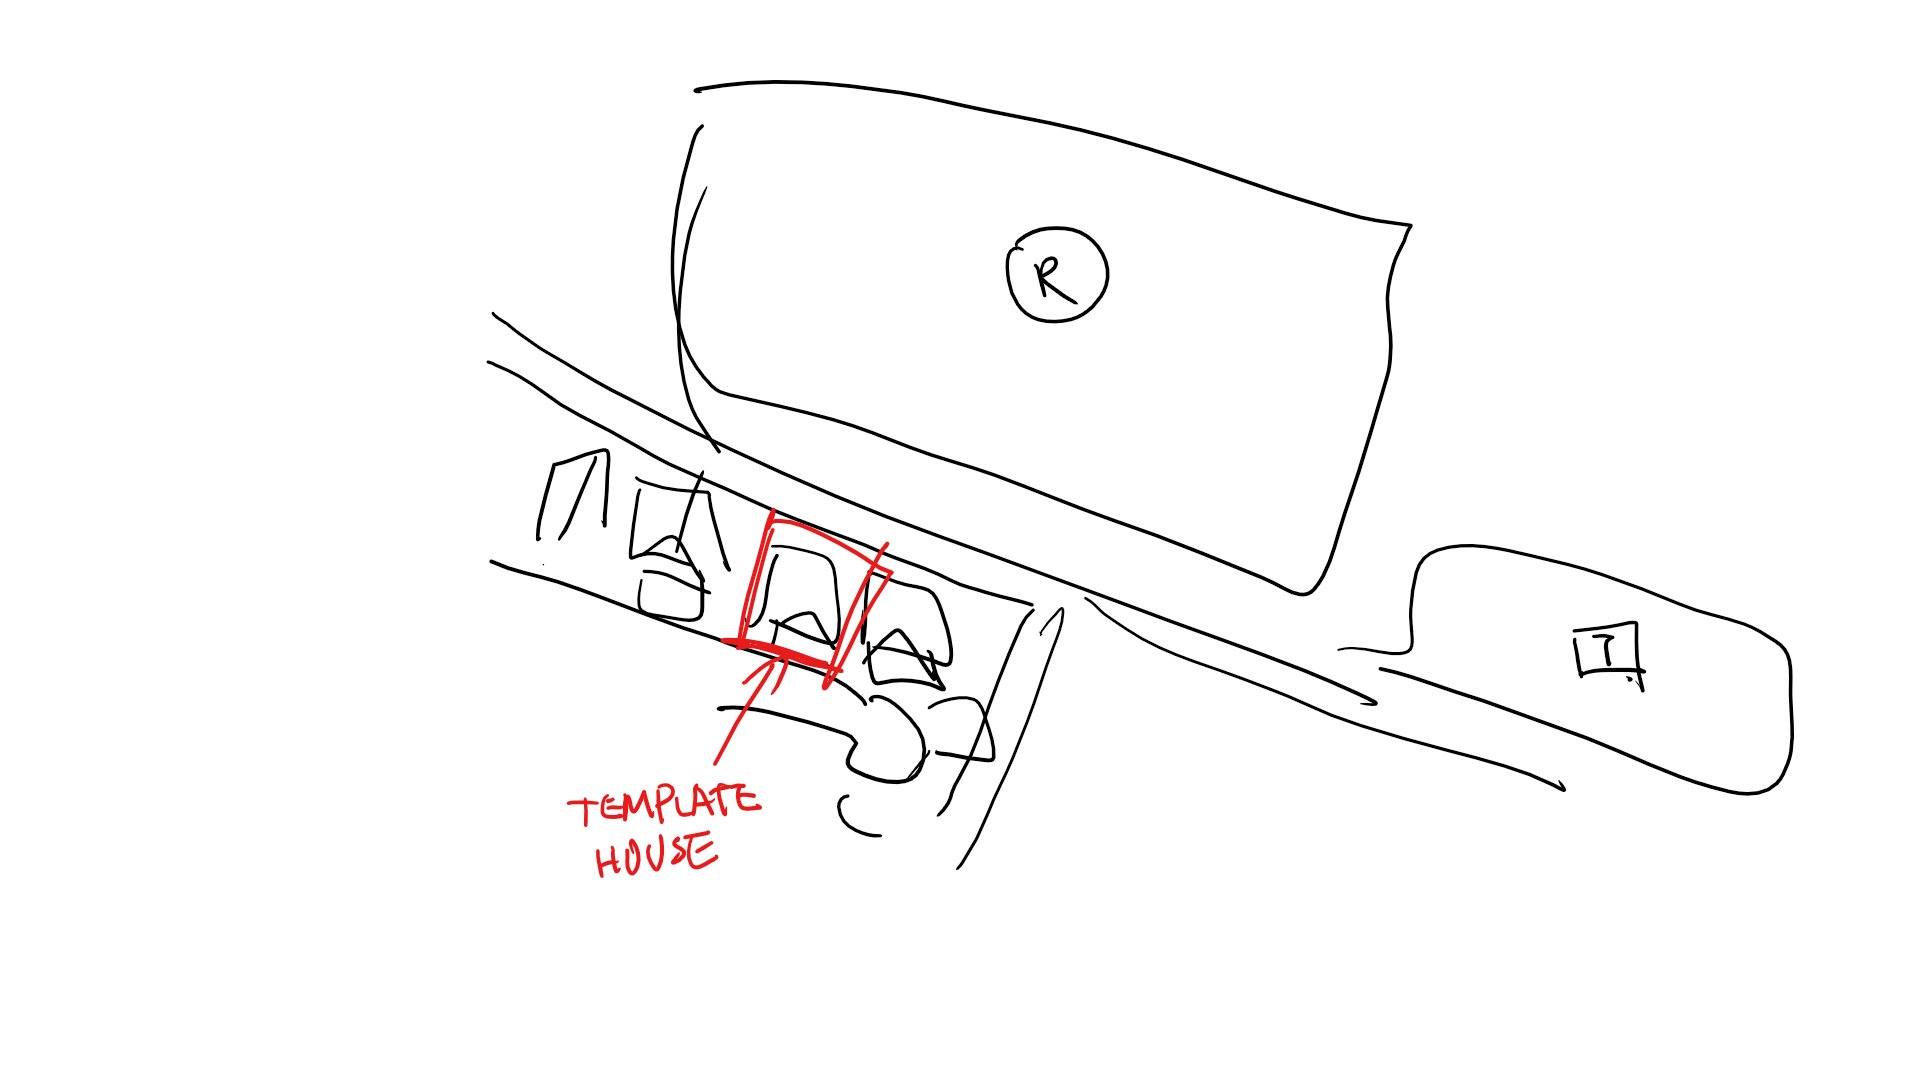
\includegraphics[width=0.6\textwidth]{assets/template-house-map}
	\caption{Map of the template house and its relative layout to the neighbourhood}
	\label{fig:template-house-path}
\end{figure}

\subsection{Requirements}\label{requriements}

The requirement is the criteria that determines if the project is a success or fail. The alternatives and layouts we consider should all meet the requirements.\\

\subsubsection{Power Demand}

The average Canadian household consumes 11,135 kWh of electricity in 2014\cite{residential-energy-use}. While Alberta household average is actually lower than the national average: at 7200 kWh. For the sake of analysis and providing a conservative estimate, we will use 8300 kWh per household.\cite{aeso-load-data, ieso-power-data, callmepower}\\

Finding the daily average, the daily energy use is given by

$$
E_\text{daily}=8300\div 365.25 = 22.7\text{kWh per day}
$$

An ideal sustainable system would need to supply at least 22.7 kWh a day on average for everyday of the year. However, we will see later in section <INSERT> that the power demand is non-uniform. On top of that, during winter times, the solar performance is hindered by the reduced hours of sunlight and snow coverage. Having big enough batteries to compensate the reduced generation for an entire season is inconceivable. This issue will be explored in more detail in the weather and geneartion section <INSERT>\\

\subsubsection{Rate of Return}

Because this is an economic analyis of a project meant to save costs in the long-run, we will assume an after-tax MARR of 3\%. This aligns with historical data from the industry.\\

\section{Scenario}

For this economic analyis, the following assumptions will be asserted. These assumptions are based off of real data.\\
\\
We will assume the solar system is installed for a residential household. Despite that, to incorporate the tax and asset analysis element in this exploration, we will treat the saved costs as operational income. The equipment will be treated as assets with the correspondant CCA class defined by the Canadian Revenue Agency\cite{cca}. As such, the assets will be depreciated by using the method outlined in the course.\\

\subsection{Energy Consumption}

As calculated earlier is the requirements subsection (section \ref{requriements}), the yearly average is 8300 kWh. The monthly average is then 692 kWh and  the daily average is 22.7 kWh. All uniformly spreadout throughout the year. To ensure the analyis is more realistic and accurate, we will tweak the usage such that it follows a cosine curve. The characterisitcs of the this consumption curve is derived from real hourly usage data collected by AESO and IESO.\cite{aeso-load-data, ieso-power-data}\\
\\
I derived a formula for monthly consumption such that the yearly average is still 8300 kWh, but the monthly usage varies due to seasonal applicance usage:

\begin{equation}
	\text{Monthly Consumption}=X\cos\left(\frac{m\pi}{6}\right)+M
	\label{eqn:monthly-consumption}
\end{equation}

Where $X$ is the expected fluctuation in consumption between the seasons. Suppose this is 10\% of monthly 692 kWh usage.\\
\\
Where $m$ is the month in numerical form (1 for January, 5 for May, etc.) and $M$ is the monthly average (692 kWh).\\
\\
The projected consumption by our model for each month is computed using equation \ref{eqn:monthly-consumption} in the table as follows (table \ref{table:consumption-table}, figure \ref{fig:consumption-graph}):

\begin{table}[H]
	\centering
	\begin{tabular}{ |c|c| }
		\hline
		Month & Consumption\\
		\hline
		1 & 751.57 kWh\\
		2 & 726.25 kWh\\
		3 & 691.67 kWh\\
		4 & 657.09 kWh\\
		5 & 631.77 kWh\\
		6 & 622.50 kWh\\
		7 & 631.77 kWh\\
		8 & 657.09 kWh\\
		9 & 691.67 kWh\\
		10 & 726.25 kWh\\
		11 & 751.57 kWh\\
		12 & 760.84 kWh\\
		\hline
		Total & 8300 kWh\\
		\hline
	\end{tabular}
	\caption{Modelled monthly electricity consumption}
	\label{table:consumption-table}
\end{table}

\begin{figure}[H]
	\centering
	
\includegraphics[width=0.6\textwidth]{assets/placeholder}
	\caption{Modelled monthly electricity consumption (graph)}
	\label{fig:consumption-graph}
\end{figure}

The full detailed calculations can be found in appendix \ref{appendix:consumption}.\\
\\
\subsection{Weather}

The biggest uncertainty lies in weather. Fortunately, Edmonton is statistically one of the sunniest places in Canada, with 4383 hours of daylight and 2205 of sunlight annually on average\cite{sunshine-canadian,climatemps}.\\
\\
Using this information, we can build a model, similar to that of the monthly consumption to determine the amount of sunlight the PV cells have exposure to.\\
\\
The output is a sinusoid with the peaks at mid-year during summer seasons: (figure \ref{fig:weather-daylight}).\\

\begin{figure}[H]
	\centering
	
\includegraphics[width=0.6\textwidth]{assets/placeholder}
	\caption{Model projection of hours of daylight monthly}
	\label{fig:weather-daylight}
\end{figure}

Daylight does not imply direct sunlight. Climatemps concludes that 50.3\% of the daylight time is sunny, 25\% is cloudy or shade, and the rest 24.7\% is other times where sun has low intensity, possibly due to rain, snow, etc\cite{climatemps}. Thus, the number of sunny hours is 50.3\% times the total monthly daylight hours. Likewise for the other two.\\
\\
Now that we classified possible weather to three general states, we can assign a relative solar performance score to each. For sunny weathers, the overall effect on the solar panel performance is minimal, the performance is expected to be at 90\%. This is not 100\% because we need to account for shallow angles of the sun during mornings and evenings. For cloudy, the performance can drop to 50\%, and lastly 25\% performance for overcasts.\\
\\
Using these statistics, we can compute the expected value of the \textit{equivalent hours of direct sunlight} received by the PV cells.

\begin{equation}
	\text{Equivalent hours}=\text{Sunny hours}\times50.3\%+\text{Cloudy hours}\times 25\% + \text{Overcast hours}\times 24.7\%
\end{equation}

We then multiply these equivalent hours by a correction factor such that the projected data will fit better than real collected data from home-owners with solar panels. These data are available from Kuby, a solar systems installation and consulting firm in Alberta\cite{kuby-complete-guide}. The correction factor corrects the loss in efficiency due to more extreme weather conditions in the winter and snow obstructions.\\
\\
The final monthly equivalent sunlight hours is shown in figure \ref{fig:weather-corrected}. This will be directly incorporated into our economic analyis to determine how much grid power we need.\\
\\
\begin{figure}[H]
	\centering
	
\includegraphics[width=0.6\textwidth]{assets/placeholder}
	\caption{Corrected equivalent sunlight hours}
	\label{fig:weather-corrected}
\end{figure}

The full detailed calculations can be found in appendix \ref{appendix:weather}.\\
\\

\subsection{Grid Power}

Using Ontario Energy Board (OEB) collected historical data for time-of-use (TOU) electricity rates as referece, we build a model for the grid power for the next 40 years\cite{oeb}. The collected data goes back to 2006 which should be enough to project a trend. Table \ref{table:grid-history} shows the electricity rates depending on TOU.\\

\begin{table}[H]
	\centering
	\begin{tabular}{|c|c|c|c|}
		\hline
		Year & Off-peak (\$/kWh) & Mid-peak (\$/kWh) &  On-peak (\$/kWh)\\
		\hline
		2006 & \$0.04 & \$0.08 & \$0.11\\
		2007 & \$0.03 & \$0.07 & \$0.09\\
		2008 & \$0.03 & \$0.07 & \$0.09\\
		2009 & \$0.04 & \$0.08 & \$0.09\\
		2010 & \$0.05 & \$0.08 & \$0.10\\
		2011 & \$0.06 & \$0.09 & \$0.11\\
		2012 & \$0.07 & \$0.10 & \$0.12\\
		2013 & \$0.07 & \$0.10 & \$0.12\\
		2014 & \$0.08 & \$0.11 & \$0.14\\
		2015 & \$0.08 & \$0.12 & \$0.16\\
		2016 & \$0.09 & \$0.13 & \$0.18\\
		2017 & \$0.08 & \$0.11 & \$0.16\\
		2018 & \$0.07 & \$0.09 & \$0.13\\
		\hline
	\end{tabular}
	\caption{Historical electricity rates}
	\label{table:grid-history}
\end{table}

Power Stream's data gives into insight into the duration of the peak times. Using that determine for each day, 50\% of the time is off-peak, 25\% of the time is mid-peak and on-peak\cite{powerstreamTOU}. Using this statistics, we find the expected value for electricity each year (equation \ref{eqn:historical-electricity}):\\

\begin{equation}
	\text{EV electricity rates}=50\%\times\text{off-peak rate}+25\%\times \text{mid-peak rate}+25\%\times\text{on-peak rate}
	\label{eqn:historical-electricity}
\end{equation}

Using past electric bills and online sources as references, there are also associated \textit{transmission, distribution}, and \textit{administration} fees associated with each kWh of consumption. Looking at a sample electric bill, the ratio of these fees, relatives to the electricity rates is as follows (table \ref{table:grid-fees}). Note that this only applies to year 2018, as projected rate of increase for electricity is different from rate of increase for distribution and transmission.\\

\begin{table}[H]
	\centering
	\begin{tabular}{|c c|}
		\hline
		Transmission&16.80\%\\
		Distribution&13.00\%\\
		Admin&5.00\%\\
		\hline
	\end{tabular}
	\caption{Rates of other electricity fees as a ratio to main electricity rates}
	\label{table:grid-fees}
\end{table}

The total cost per kWh for 2018 is \$0.1165 per kWh.\\
\\
We assume the projected increase in electricity rates is 5.10\% annually, and the projected rate of increase for transmission and distribution is 2.20\% annualy.\cite{transmission-projection} Using the 2018 rates as base rate, we can compute the cost at some future time. Figure \ref{fig:grid-projection} shows tThe estimated trajectory of grid electricity costs. Full calculations and tables can be found in appendix \ref{appendix:grid}.

\begin{figure}[H]
	\centering
	
\includegraphics[width=0.6\textwidth]{assets/placeholder}
	\caption{Projected total cost to electricity per kWh}
	\label{fig:grid-projection}
\end{figure}

According to BCHydro, the current buyback rate for excess generated electricity is 9.99 cents per kWh\cite{bchydro-buyback}, assume a slow but steady growth of 1.0\% a year. The buyback rate could be directly incorporated into our analysis (figure \ref{fig:grid-buyback}).

\begin{figure}[H]
	\centering
	
\includegraphics[width=0.6\textwidth]{assets/placeholder}
	\caption{Projected buyback rate for electricty per kWh}
	\label{fig:grid-buyback}
\end{figure}

\subsection{Government Incentives}

Asides from saving money in the long-run and potentiall selling excess energy (see previous section for buyback), the Alberta government and the City of Edmonton offers generous incentives that takes form of a one-time rebate.\cite{kuby-costs,kuby-edmonton,kuby-alberta}\\
\\
The rebate is applied immediately when the project is purchased with cash, or applied immediately and reduces the debt if a loan is taken.\\
\\
Alberta offers a rebate of \$0.75 per W, up to the lesser of \$10,000 or 30\% of the initial cost\cite{kuby-alberta}. The city of Edmonton offers an additional \$0.15 per W, no upper limits.\\

\subsection{Capital}

There are two main methods of purchasing, cash or loan. For the sake of simplicity, we will assume it is one or the other. We will also assume we have less than \$10,000 of savings immediately in savings. This implies that any setup under the cost of \$10,000 can be paid in cash.\\
\\
Otherwise, we can choose to take a loan. The details for the loan is up to the contractor. This will be specified in the differente alternatives in the alternatives section (section \ref{section:alternatives}).\\
\\
For loans, it is commonly to be relative to a \textit{prime rate}. In this case, we use the recent data from yCharts which shows 3.0\%.\cite{prime-rate} We assume that this rate won't change.\\
\\
Finally, we will use a conservative constant 2\% annual inflation rate based on historical data.\cite{inflation} We assume this rate do not change for the duration of the analysis.\\

\subsection{Depreciation and Taxes}

Since we treat the cost savings as a business income, they will be taxed like a business. The corporation tax for new, small businesses is 10\% according to the Revenue Agency\cite{business-tax}.\\
\\
Any non-contracted purchases will be subject to a local sales tax GST of 5.0\%.\\
\\
Purchases that has a defined CCA class will be added to a UCC account. The book value for that account will be depreciated by the corresponding CCA class rate. In this analysis, we conservatively assume that excess tax credit are not carried on to the next year, and that the government will not provide negative tax (positive cashflow).\\

\subsection{Maintainance}

\subsection{Salvage}

\section{Alternatives}\label{section:alternatives}

TODO:\\
\\
Here I will select a few alternatives given by choosing the parameters outlined in the previous section (section \ref{section:parameters}) and use them as possible alternatives. The do-nothing alternative is implied by selecting 0 solar panels, 0 batteries, and no auxillery upgrades.\\

\section{Economic Model}
As briefed explained in section \ref{subsection:rcgs}, the economic model will be a combination of segmenting model, where the cashflows are broken into differet core components, learning curve model (for modelling the effective of technlogy and repetitive installation). Finally, the cost index model for market prices of products.\\

\subsection{Expected Cashflow-In}
The main benefit or positive cashflow is from the savings in electrical bills. We would also need to analyze the current and projected future cost to electricty from utility companies. Note that electricity costs may even change throughout the year as demand changes.\\
\\
There are various other ways that would invoke a positive cash flow:\\

\begin{itemize}
	\item Alberta government incentives that promotes green energy; they provide a fixed cash-back from receipts of purchases of renewable technologies. This will be a one-time / non-recurring benefit.

	\item Extra, unused power may be sold back to utility companies; they could also be redirected to other households whose demands are higher.

	\item Salvage value for the technologies and equipment at the end of analysis period. If well-maintained, there should be a high resale value as demand for renewable equiment increases in time.
\end{itemize}

\subsection{Expected Cashflow-Out}\label{subsection:cashflow-out}

We should expect majority of the cost will be the initial cost of equipment and installation.\\
\\
If the solar panels or installation is financed, then the initial cost would be the down-payment. However, we would also expect a debt with interest $i$. This will ultimately affect our MARR in our rate of return analysis (section \ref{subsection:rate-of-return}).\\
\\
Post-installation, there will be periodic cost to maintain the equipment. The solar panels would only need to be cleaned, and replacement is only necessary when the cells fail, which has low probability. Another periodic cost would be replacement of the batteries. Eventhough the batteries are rechargeable, they have about 5,000 full charge cycles while their effective performance and capacity decrease over time\cite{tesla-powerwall-wiki}.\\

\subsection{Sources of Capital}

For minimum risk in rate or return, all funding will come from other family members taking dividends in the project. The source of capital will be our savings and income.\\
\\
Alternatively, to put on less pressure financially in present time, we could choose to take out a one-time loan to pay all project costs up-front. The interest rate $i$ of the loan will mostly drive the MARR in the rate of return analysis (section \ref{subsection:rate-of-return}).\\
\\
Lastly, we could choose not to take loan, but finance the cost to install assuming that such option is available. Again, as mentioned in section \ref{subsection:cashflow-out}, the interest rate of the financing plan will affect the MARR.\\

\subsection{Taxes}
\begin{center}
	This section is intentionally left blank (haven't covered there in the course yet).\\
\end{center}

\section{Analysis}

We will run the analysis period for three time-scales: 

\begin{itemize}
	\item short-term (5 years) - appropriate for if we don't stay at the house very long (such as for when the house gets sold or rented out). Since 5 years is short, it's likely that the equipment and technology are not yet obsolete. Thus for this analysis period, we would account for the extra salvage value / resale value at the end of the 5 year period.\\

	\item medium-term (20 years) - this is the most realistic time period for most home-owners. The projection of power company electricity costs will be estimated using cost-index. The improvement in technlogy for the replaced solar panels are modelled as learning curve model.\\

	\item long-term (40 years) - this analysis period is appropriate for long term residency. The market price, cost index, and technology efficiency would be quite inaccurate in the far future. The assumption is that we would still be using the same system.
\end{itemize}

\subsection{Net Present Value Analysis}

For each of the three analysis periods, a net present value analysis will be performed. The assumption is that everything is re-purchaseable. The cost of replacement will follow a model based on the cost index trends.\\
\\
The NPV should infer roughly a good solution.\\
\\

\subsection{Equivalent Annual Cashflow Analysis}
The different alternatives would have different lifetimes and replacement would be required. We will consider \textbf{Replacement analysis}. When the old panel become so inefficient that the equivalent annual cost to operate the old panel (including the extra cost paid to the power companies) is greater than the equivalent annual cost of buying and operating new panels.\\

\subsection{Rate of Return Analysis}\label{subsection:rate-of-return}
Here we will compute the IRR of the given alternatives for all three analysis periods.\\

\section{Simulation}

The simulation will run for all three proposed analysis periods. For the 5 year perio, historical weather data will be collected and ran through the simulation. For 20 and 40 years, based on historical data, random weather conditions will be generated.\\
\\
These simulations will serve as a resiliency test, and the final cost at the end of the simulation period will be compared amongst the alternatives.\\

\section{Sensitivity and Risk Analysis}

After initial simulation, individual parameters such as compass-heading of the house, climate conditions, etc. will be altered to the simulation. This will yield how much the NPV or ECAF will change with respect to these alterations.\\

\section{Non-Economic Factors}
\subsection{Challenges}
- Alberta population's main economic driver is still fossil fuel, the public perception and public interst is not as sustainable as we preferred. This leads to lower supply of sustainable technlogies such as solar panels which drives up the price.\\

\section{Conclusion}\label{section:conclusion}

\subsection{Verdict}

% Bibliography
\clearpage
\addcontentsline{toc}{section}{References}
\bibliographystyle{ieeetr}
\bibliography{references}

% Appendix
\clearpage
\appendix
\section{Consumption Calculations}\label{appendix:consumption}
\begin{figure}[H]
	\centering
	
\includegraphics[width=1\textwidth]{assets/placeholder}
	\caption{Spreadsheet calculations on power consumption}
\end{figure}

\clearpage
\section{Weather Calculations}\label{appendix:weather}
\begin{figure}[H]
	\centering
	
\includegraphics[width=0.6\textwidth]{assets/placeholder}
	\caption{TODO}
\end{figure}

\clearpage
\section{Grid Calculations}\label{appendix:grid}
\begin{figure}[H]
	\centering
	
\includegraphics[width=0.6\textwidth]{assets/placeholder}
	\caption{TODO}
\end{figure}

\end{document}